
\chapter{提案}
\label{chap:suggestion}

この章では、ARを用いた生活の簡素化支援システムについて提案し、その具体的な用途について、各例ごとに考察する。

\newpage

\section{ARを用いたモノの仮想的代替による簡素化支援システムの提案}
\label{chap:suggestionDetail}

\subsection{概要}

簡素化支援システムとは、生活を簡素化のために排除したモノをARで仮想的に再現し、その代替として利用することで、簡素化前と同程度、或いはそれ以上に充実した機能を得ることができる、実世界を代替するインターフェースである。

なお、充実した日常を過ごせる部屋環境の形成には、ARでの仮想的な代替が不可欠なため、常にARデバイスを使用し続ける事を前提としている。

\subsection{仮想的な代替が可能なモノ}

人や物体の支えとなるモノや、温度を制御する機能を持つモノなど、その物体がその場になくては役割を果たせないモノかどうかで判別する。下記の表の各欄には、一般的な部屋内のモノについて、対象の物体がその場になくては役割を果たせないモノかどうかを分類している。

\begin{table}[htbp]
    \caption{物体がその場になくては役割を果たせないものかどうか}
    \label{tb:mono}
    \begin{center}\begin{tabular}{c|c}
      \hline
      果たすもの&机・椅子・本棚・タンス・冷蔵庫・洗濯機・エアコン etc..\\\hline
      果たさないもの&テレビ・時計・PCディスプレイ・カレンダー・ポスター etc..\\\hline
    \end{tabular}\end{center}
\end{table}

簡素化支援システムでは、後者に分類された物体を実世界で配置する代わりに、ARを用いて仮想的に表示することにより、生活の機能充実を損なわずに、実世界の空間の簡素化を実現する。

\subsection{使用するARデバイスについて}
\label{chap:ARdevice}

簡素化支援システムは、日常的に利用される前提のため、デバイスについても同様に日常的に使用できることが条件となる。現段階では、ARグラスがその条件を満たしている技術となっていると推察される。ARグラスとは、実世界に重ねて描画できるグラフィックデバイスで、実世界を認識して得た情報を元に様々な表示をする眼鏡型のデバイスである。代表的なARグラスとして、Hololens\footnote{Microsoft Hololens: \url{https://www.microsoft.com/ja-jp/hololens}(accessed 2021-01-26)}、Magic leap 1\footnote{Magic leap 1: \url{https://www.magicleap.com/ja-jp/magic-leap-1} (accessed 2021-01-26)}、Nreal light\footnote{Nreal light: \url{https://www.nreal.ai/light/} (accessed 2021-01-26)}などがある。いずれもPCを必要とせず、スタンドアロンで動作する。空間に対する位置・角度などを検知できるため、6DoF(six degrees of freedom)に対応しており、高い没入感を得ることができる。

\newpage

\section{簡素化支援システムの具体的なシナリオの考察}

ここでは、\ref{chap:suggestionDetail}にて挙げた生活の簡素化支援システムについて、より具体的なシナリオを交えた上で、多角的に考察する。

\subsection{部屋の空間の確保と機能性の拡張}

\ref{chap:ARdevice}で提示した、仮想的な代替が可能なモノを、部屋から排除することにより、空間の確保をすることができる。確保した空間には、ARで再現したモノを表示するが、状況に応じて非表示にしたり、別のモノを表示することも可能なため、より自由度の高い空間にすることが可能である。

ARによって仮想的に表示しているため、物理法則に囚われない表示をすることも可能である。壁や天井などは空きスペースとなっている場合が多いが、そういった箇所も有効活用する事が可能である。

また、元々部屋になかったモノの配置をすることで、部屋の機能をより充実させることができる。例えば、スマホウィジットに代表される、時間、天気やカレンダー、todo、体調状態、メモ、その他情報なども配置することができ、部屋をスマートフォンのホーム画面のように利用する事も可能である。なお、スマートフォンでの時刻や日付の確認が容易になった現代でも、カレンダーや時計を部屋に配置する事と同様に、これらの情報を部屋内で見られるようにすることで、部屋内の相対位置によって機能の場所を記憶することが容易となり、欲しい情報を瞬時に獲得、もしくは機能を利用する事ができるのではないかと推察する。

\begin{figure}[htbp]
    \begin{minipage}{0.5\hsize}
      \begin{center}
        \fbox{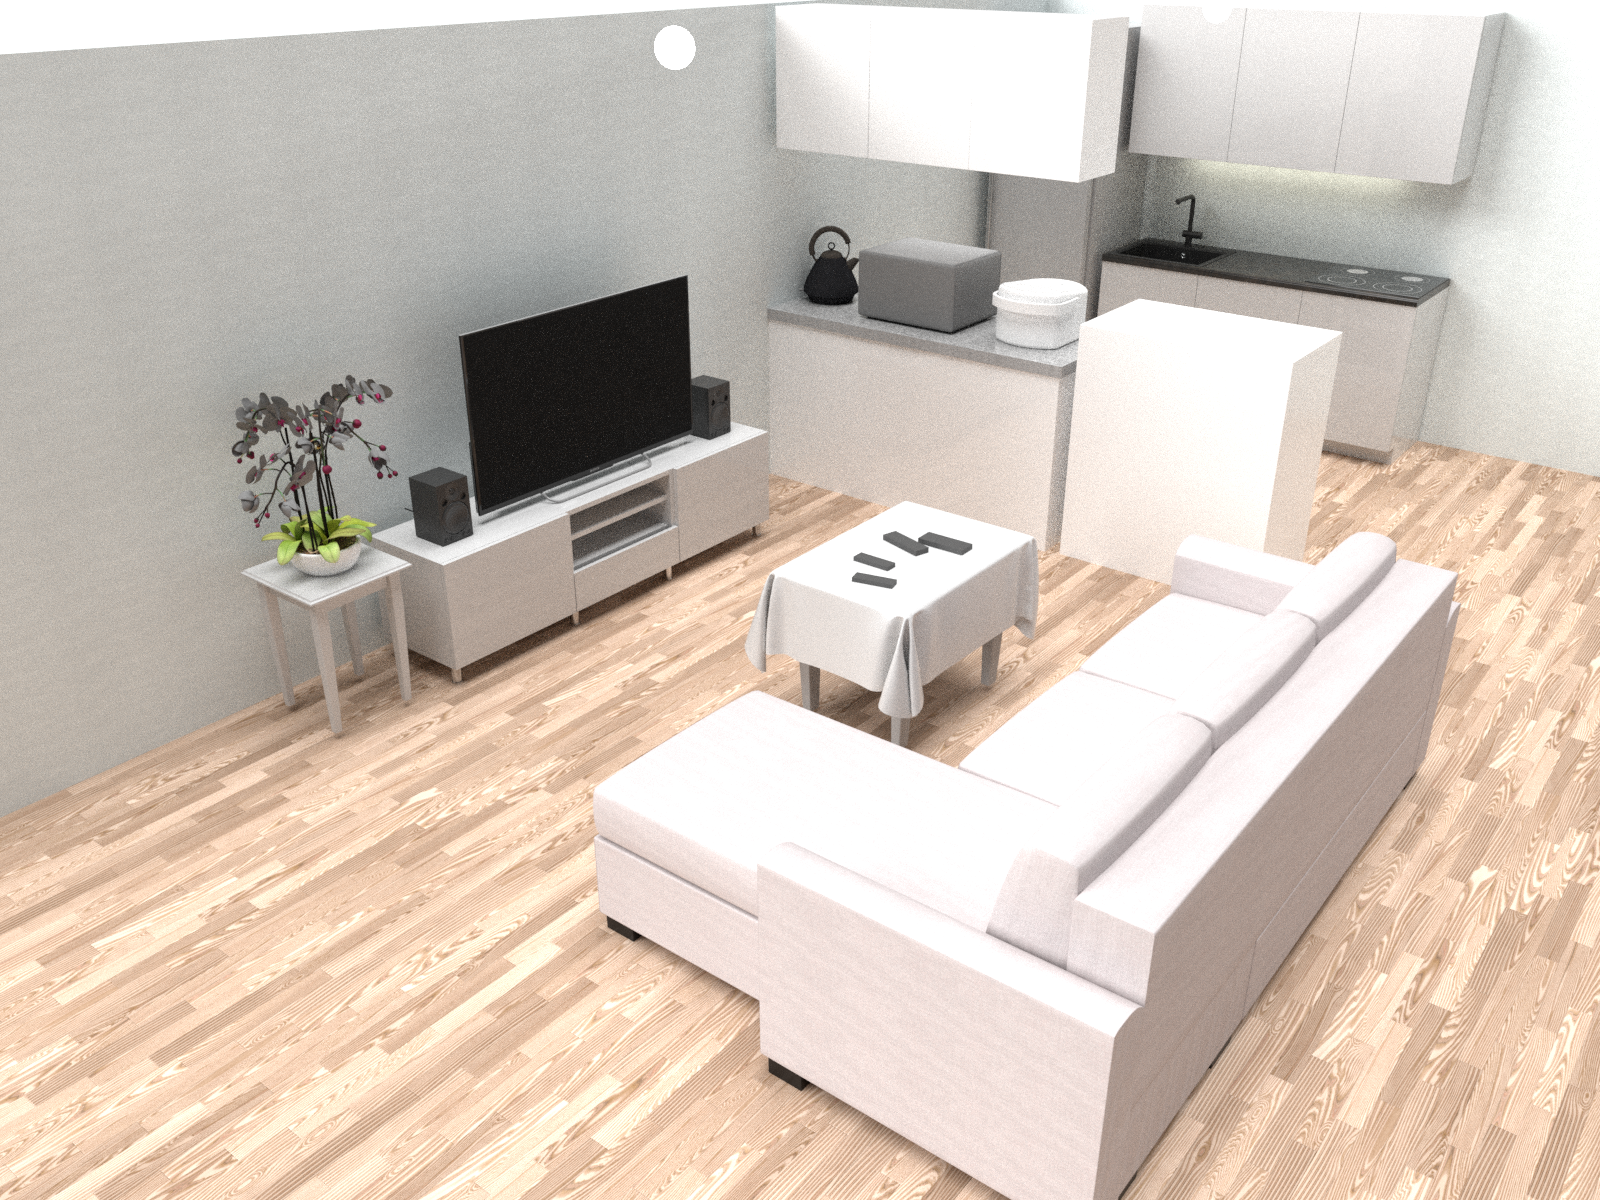
\includegraphics[width=60mm]{images/living_room_01.png}}
      \end{center}
      \caption{通常の部屋環境のイメージ}
    \end{minipage}
    \begin{minipage}{0.5\hsize}
      \begin{center}
        \fbox{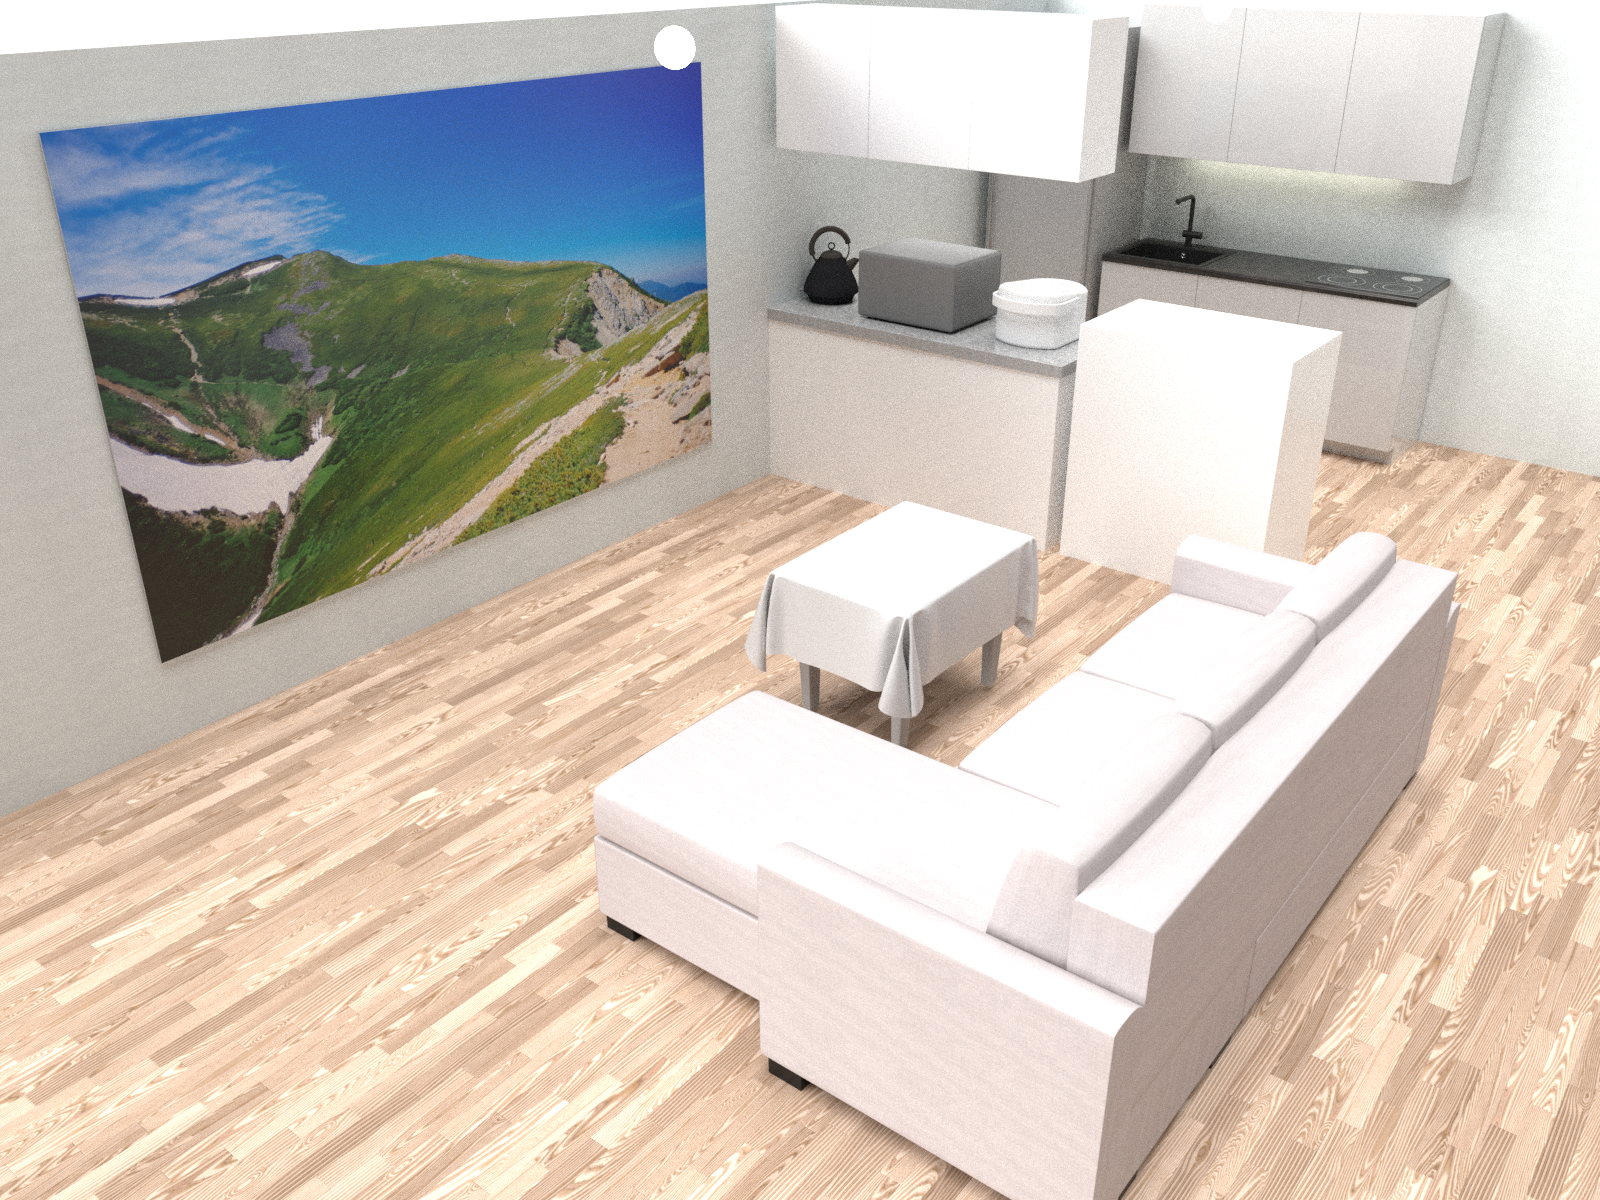
\includegraphics[width=60mm]{images/living_room_02.png}}
      \end{center}
      \caption{テレビを排除し仮想的に代替したイメージ}
    \end{minipage}
  \end{figure}

\subsection{同様の環境を他所で再現}

自身が身を置く場所は常に一定ではなく、自宅の部屋以外にも、オフィスやカフェ、ホテルなどのシチュエーションに身を置くこともある。その際に、本システムを利用する事で、普段とは違う場所でも、自室の環境を再現することができる。

また、逆に、他所の部屋環境を、自身の部屋環境として再現することも可能である。オフィスや映画館など、シチュエーションに応じたモノの再現が可能なため、より個人の充実に適した環境を用意することができる。

\subsection{物体の管理や更新、カスタマイズ}

物体としての実体を持たないので、購入や修理などのコストがかからない。また、物体の更新にも物理的なコストは掛からないので、色や形、大きさまで、自由にカスタマイズすることができる。

